% Created 2022-04-18 Mon 10:29
% Intended LaTeX compiler: pdflatex
\documentclass[10pt,t]{beamer}
\usepackage[utf8]{inputenc}
\usepackage[T1]{fontenc}
\usepackage{graphicx}
\usepackage{grffile}
\usepackage{longtable}
\usepackage{wrapfig}
\usepackage{rotating}
\usepackage{amsmath}
\usepackage{textcomp}
\usepackage{amssymb}
\usepackage{capt-of}
\usepackage{hyperref}
\usetheme{default}
\author{L. Larrabee Strow}
\date{\today}
\title{\large Satellite Hyperspectral Infrared Climate Time Series Combining AIRS and CrIS}
\subtitle{\footnotesize{Sun-Climate Symposium}}
\date{\vspace{0.1in}\footnotesize{May 18, 2022 \vfill}}
\author{L. Larrabee Strow\inst{1} and Sergio DeSouza-Machado\inst{1}}
\institute[UMBC]{\inst{1} UMBC Physics Dept.}
\input beamer_setup
\usetheme{metropolis}
\metroset{titleformat title=allcaps}
\renewcommand{\UrlFont}{\small\tt}
\renewcommand*{\UrlFont}{\footnotesize}
\tolerance=1000
\begin{document}

\maketitle
\begin{frame}[label={sec:org78d47e3}]{Introduction}
\vspace{-0.15in}
\small
\begin{itemize}
\item Climate monitoring requires proven stability with high accuracy and/or sensor overlap

\item Focus on simple retrieval approaches that are connected as closely as possible to the measured radiances and are amenable to frequent reprocessing

\item We hope to show that hyperspectral IR radiance analysis provides important measurements of climate, with minimal a-priori information

\item Fusion with different remote sensing data type can reveal null space error in both, allows corrections for both sensor types (GPSRO, MLS, Imagers, etc.)
\end{itemize}

\vspace{-0.15in}
\rule{\linewidth}{0.01in}
\vspace{-0.2in}

\footnotesize
No discussion of  existing cloud retrievals using IR (eg B. Kahn, Claudia Stubenrauch), or minor gas or 
dust/ash retrievals using IR.   \\
\vspace{0.03in}
Thanks to Howard Motteler, Chris Hepplewhite, and Ryan Kramer (UMBC) and Stephen Leroy (AER)
\end{frame}

\begin{frame}[label={sec:orgfe24b29}]{Satellite Measurements: \small \textasciitilde{}12-km footprints, full coverage 2X/day}
\begin{center}
\begin{tabular}{lll}
AIRS & 2002 - 202X?? & 1:30 orbit\\
\hline
CrIS & 2012 - 204X? & 1:30 orbit\\
\small 1 SNPP-CrIS, 4 on JPSS &  & \\
\hline
IASI & 2007 - 204X? & 9:30 orbit\\
\small 3 on METOP-A series &  & \\
\small 3 on METOP-SG series (2024) &  & \\
\small(IASI-1 CDR available on request) &  & \\
\hline
CHIRP (AIRS+CrIS) & 2002 - 204X & 1:30 orbit\\
\small "Virtual" L1c for climate &  & \\
\end{tabular}
\end{center}

Each sensor produces \textasciitilde{}2-3 million observations (spectra) daily. \\
\vspace{0.1in}
%AIRS needs reprocessing to CDR (Climate Data Record) level to fix small calibration issues.
\end{frame}

\begin{frame}[label={sec:orga727ef9}]{Example Spectra}
\begin{center}
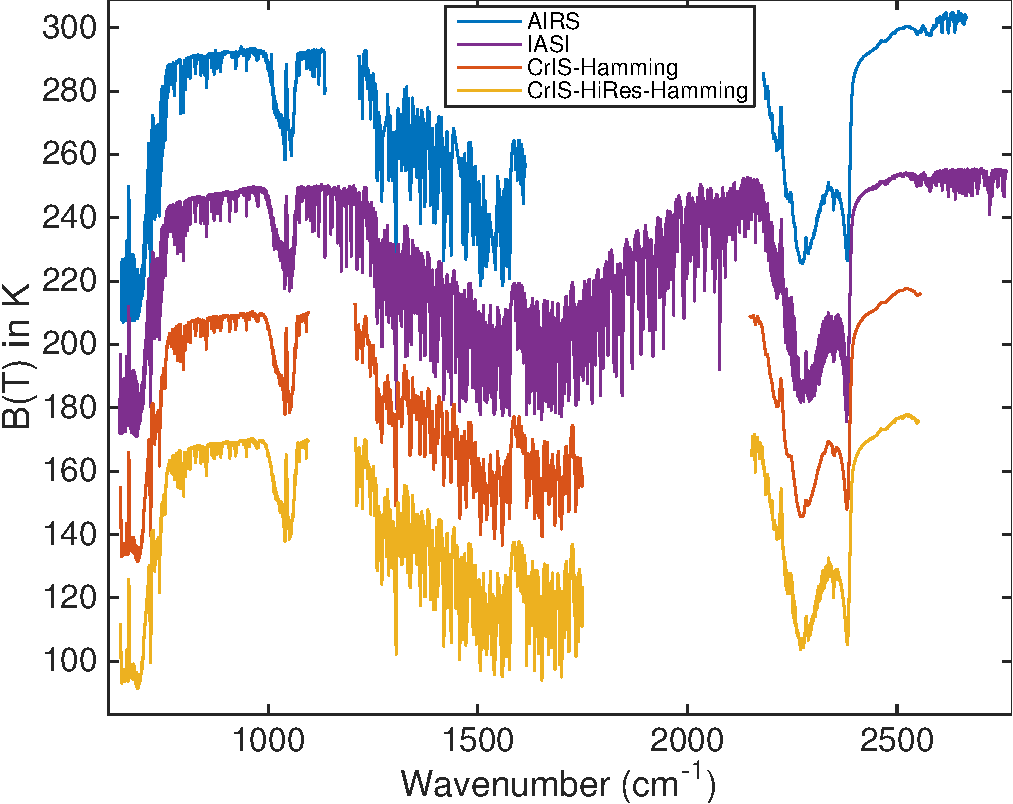
\includegraphics[width=0.9\linewidth]{Strow_JPL_Apr2022/jpl_min//hyperall_hamming.pdf}
\end{center}
\end{frame}

\begin{frame}[label={sec:org409554b}]{Overall Approach}
\begin{itemize}
\item Driven by Level 2 + Time \(\neq\) Climate
\item Full sampling not required for climate
\item Manipulate data in radiance space "as long as possible" before retrievals
\item Reduce sensitivity to calibration and RTA bias (radiance anomalies)
\item Optimal estimation retrievals regularized more by smoothing than a-priori
\item Develop analysis approaches that encourage more researchers to use radiances, rather than complicated Level 2 products for climate research, with quick turnaround.
\end{itemize}
%Working to provide CHIRP data on GES DISC AWS Cloud storage in format that allows high-speed I/O for end-user processing of radiances.
\end{frame}

\begin{frame}[label={sec:orgf6503b1}]{AIRS Stability Validation (Clear Ocean Scenes Time Series)}
\vspace{-0.1in}
\begin{center}
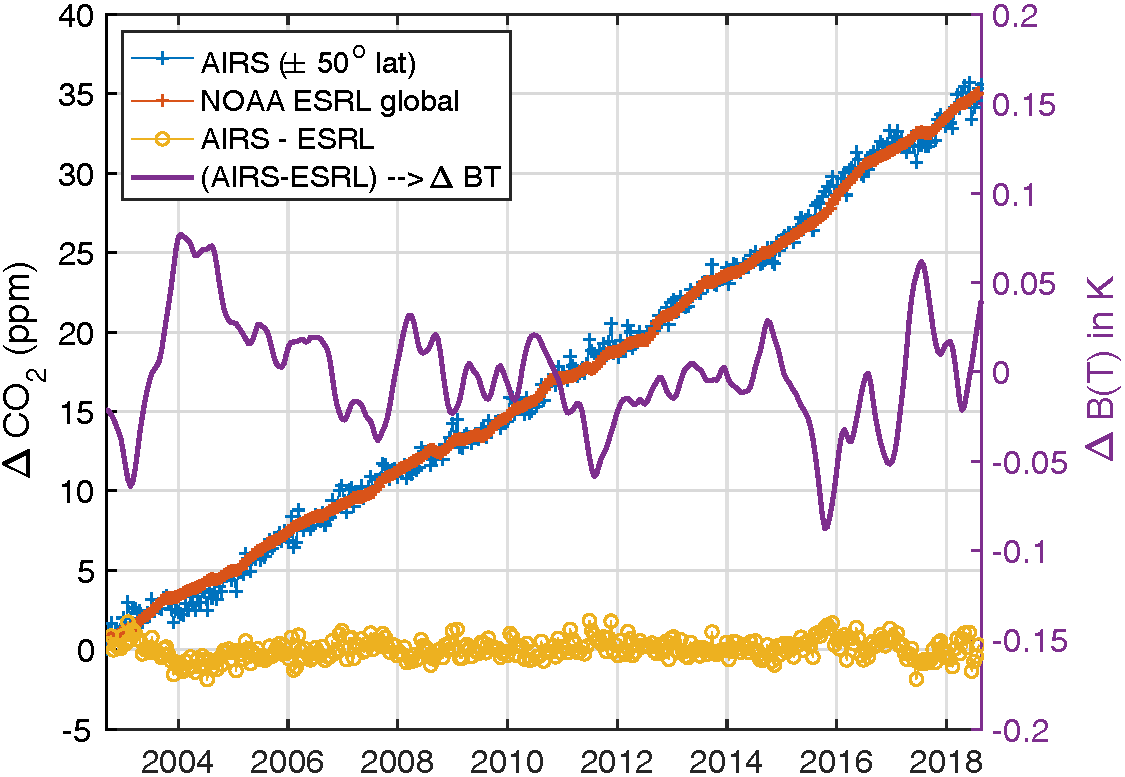
\includegraphics[width=0.65\linewidth]{Strow_JPL_Apr2022/jpl_min//yung/Figs/Pdf/fig10.pdf}
\end{center}

\vspace{-0.05in}
\footnotesize
\begin{itemize}
\item \cd trend (using 400 "good" channels) suggests stability:  -0.023 \textpm{} 0.009 K/decade.  Picks up ENSO related variations in \cd growth at the 0.04K with good S/N
\item \methane and \nitrous trends exhibit small offsets (known events, fixable)
\item (AIRS - GHRSST) SST trends:):  -0.022 \textpm{} 0.012 K/decade
\item This approach provides strong evidence of inherent radiometric stability at the climate level
\end{itemize}
\end{frame}

\begin{frame}[label={sec:orgc786a39}]{Radiance Sampling}
\begin{itemize}
\item Early testing shows identical surface T trends with 1\%, 3\%, 5\%, and 10\% hottest scenes per 16-day gridded lat/lon cell (3x5 lat/lon).
\item Will this sampling provide accurate profile trends?
\item Careful sampling of cloudier scenes does not preclude retrievals, just more care in cloud parameter a-priori values and parameterization
\begin{itemize}
\item Hyperspectral IR retrievals really need footprint matched cloud parameters from MODIS (like CERES uses).  Univ. Wisconsin has already generated this product for CrIS from VIIRS!
\end{itemize}
\item Subsequent results used 3\% surface T sampling (from 1231 \wn channel)

\vspace{0.1in}
\end{itemize}

Trend retrievals in next few slides take \textasciitilde{}1 hour max, so reprocessing is trivial.\\
  \vspace{0.1in}
Resampling (say for fixed cloud forcing) takes \textasciitilde{}2 days.  
\end{frame}

\begin{frame}[label={sec:org58f619b}]{Global IR Radiance Trends and Surface-T Anomalies}
\vspace{-0.35in}

\begin{columns}
\begin{column}{0.55\columnwidth}
\begin{block}{\footnotesize Global Trends: Clear vs All-Sky}
\vspace{-0.1in}
\begin{center}
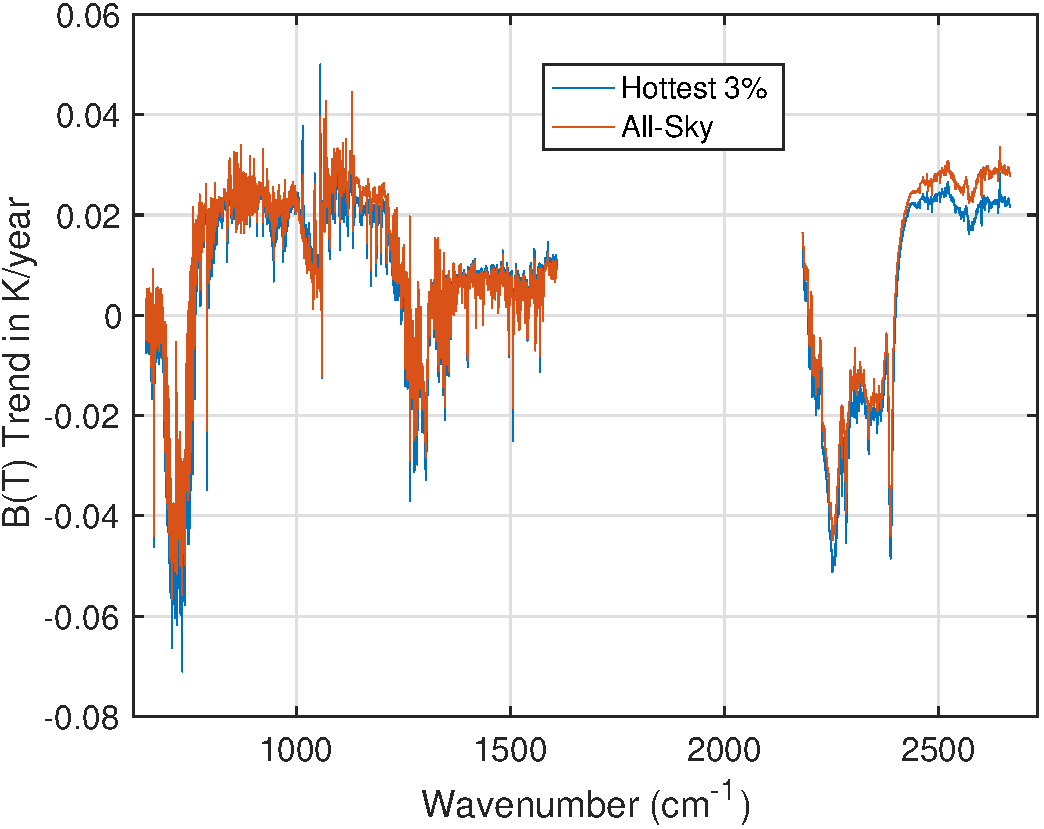
\includegraphics[width=\linewidth]{Strow_JPL_Apr2022/jpl_min//Figs1/Pdf/global_trends_hottest3pc_and)allsky.pdf}
\end{center}
\end{block}
\end{column}


\begin{column}{0.5\columnwidth}
\begin{block}{\footnotesize Tsurface Global Anomaly}
\vspace{-0.05in}
\begin{center}
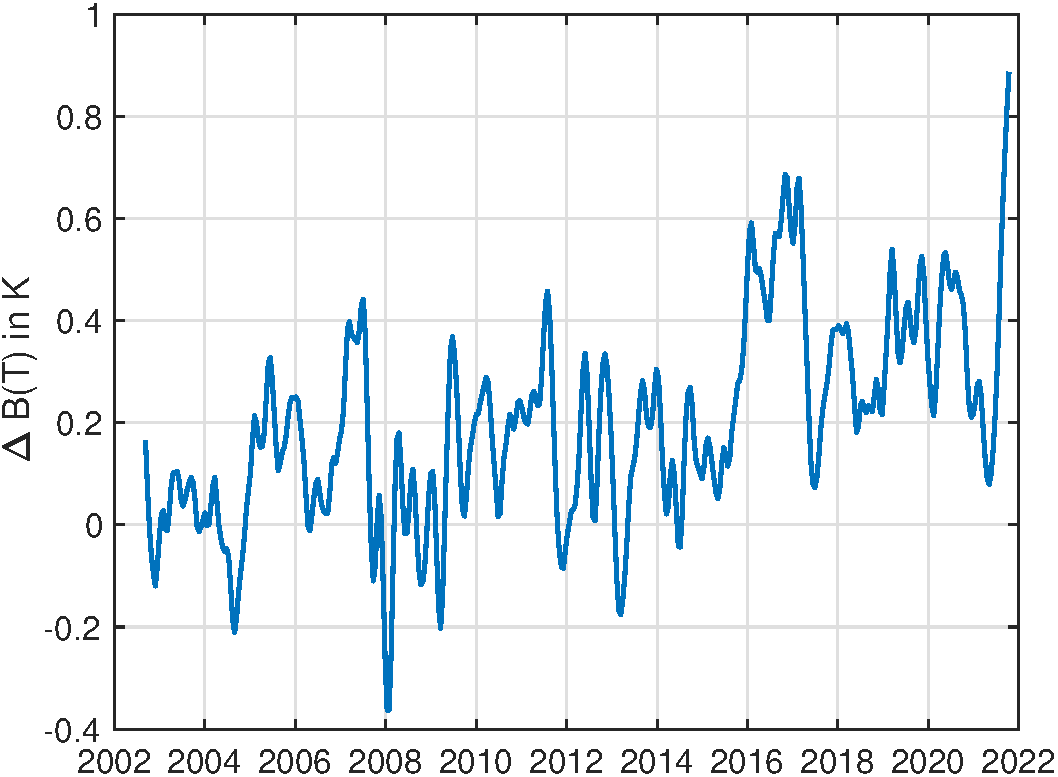
\includegraphics[width=\linewidth]{Strow_JPL_Apr2022/jpl_min//Figs1/Pdf/global_bt1231_anomaly.pdf}
\end{center}
\end{block}
\end{column}
\end{columns}

\vspace{-0.1in}
\small
\begin{itemize}
\item "Clear" 3\% hot sampling trends almost same as all-sky
\item Zonally averaged uncertainties (inter-annual variability) \textasciitilde{}0.05K/Decade
\item Good AIRS channels: stability \textasciitilde{}0.02K/Decade
\item Some water band drifts of up to \textasciitilde{}0.04K/Decade (can be fixed)
\item Shortwave known drifts (higher for cold scenes)
\end{itemize}
\end{frame}


\begin{frame}[label={sec:org2c94097}]{Follow-On Sensor: SNPP CrIS 8-Year Trends}
\begin{center}
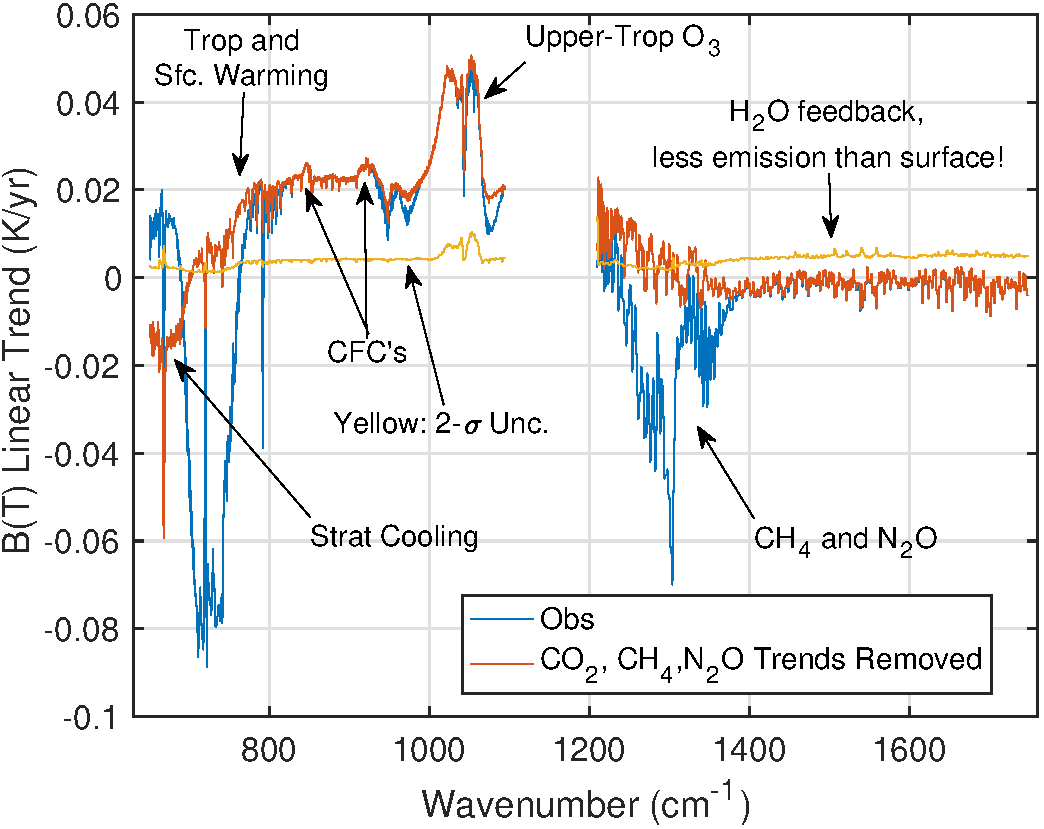
\includegraphics[width=0.8\linewidth]{Strow_JPL_Apr2022/jpl_min//Figs/Pdf/cris_dbt_clear_all_lats_lwmw_annotated.pdf}
\end{center}

\vspace{-0.1in}
\footnotesize Clear ocean scenes \\
\footnotesize Less "hash" due to nature of FTS instrumentation
\end{frame}

\begin{frame}[label={sec:orge4ee1be}]{Surface Temperature Trend Comparisons}
\vspace{-0.15in}
\begin{center}
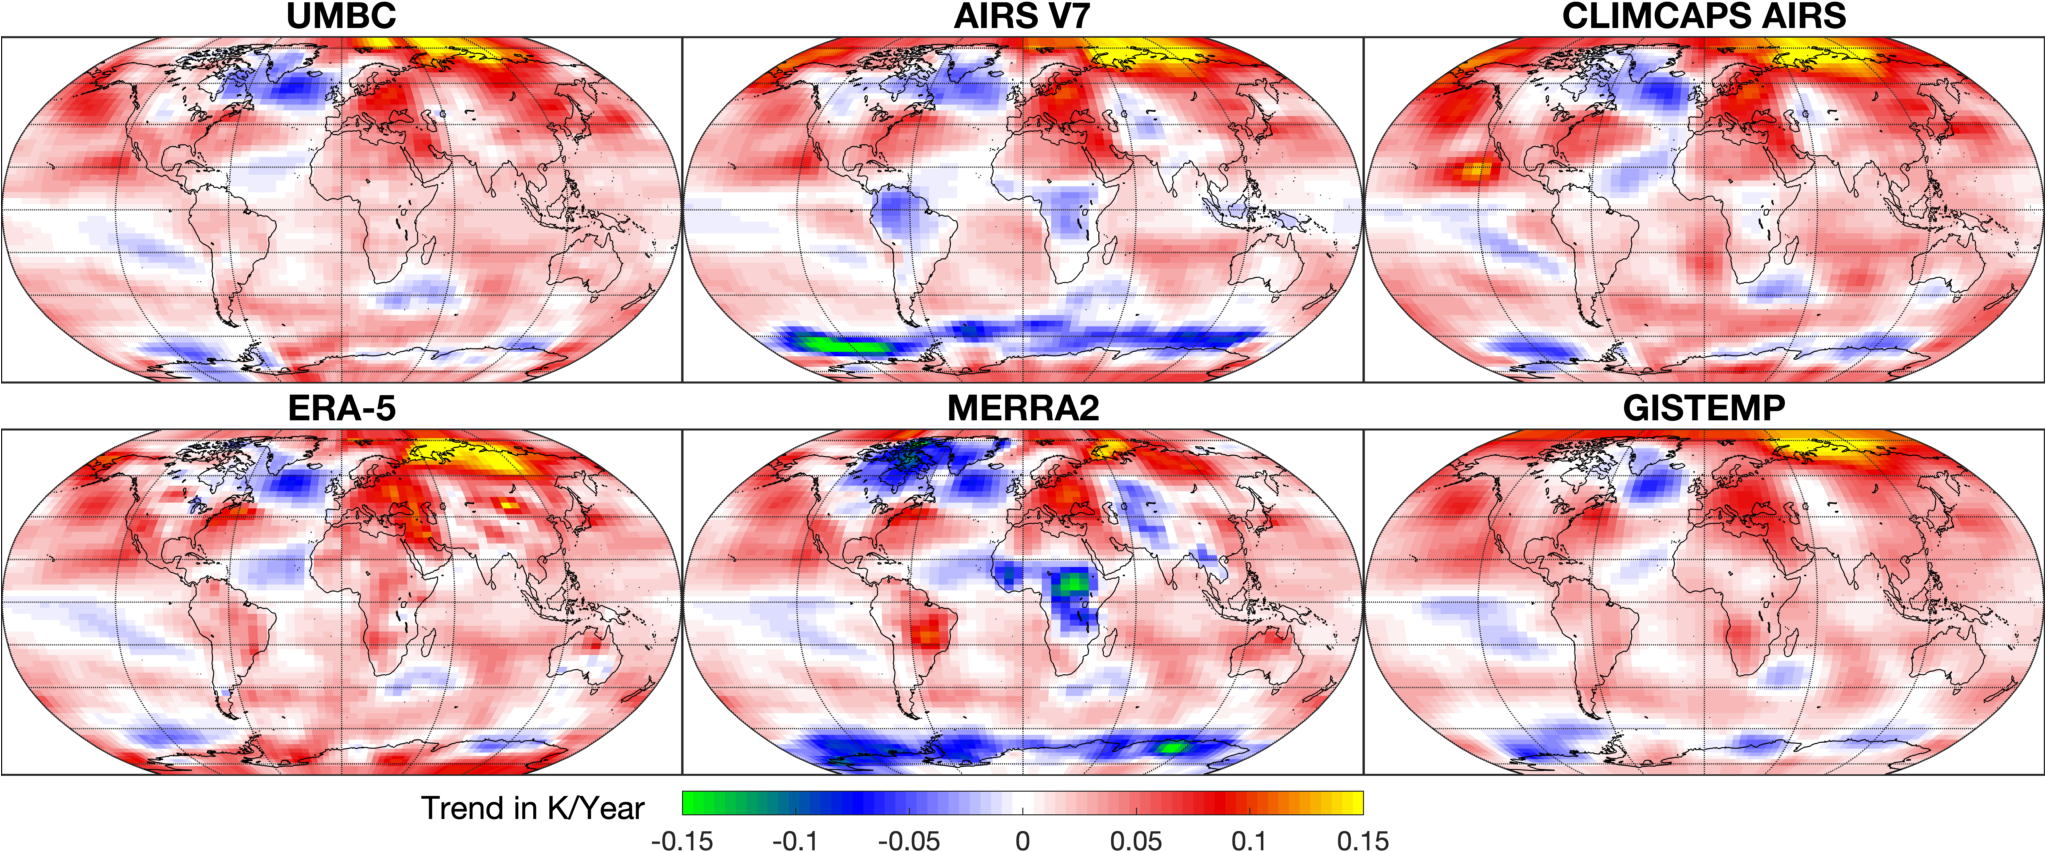
\includegraphics[width=\linewidth]{Strow_JPL_Apr2022/jpl_min//Figs/Png/tsurf_maps_6sources_giss.png}
\end{center}

\vspace{0.1in}
\footnotesize
\begin{center}
\begin{tabular}{lr}
\hline
Data Source & Spatial Correlation\\
 & (w/ UMBC)\\
\hline
CLIMCAPS AIRS & 0.82\\
GISTEMP & 0.74\\
AIRS V7 & 0.70\\
ERA-5 & 0.66\\
MERRA2 & 0.53\\
\hline
\end{tabular}
\end{center}
\end{frame}

\begin{frame}[label={sec:org4c23670}]{Zonal T(z) Trends (with CMIP6 to 2014)}
\vspace{-0.15in}
\begin{center}
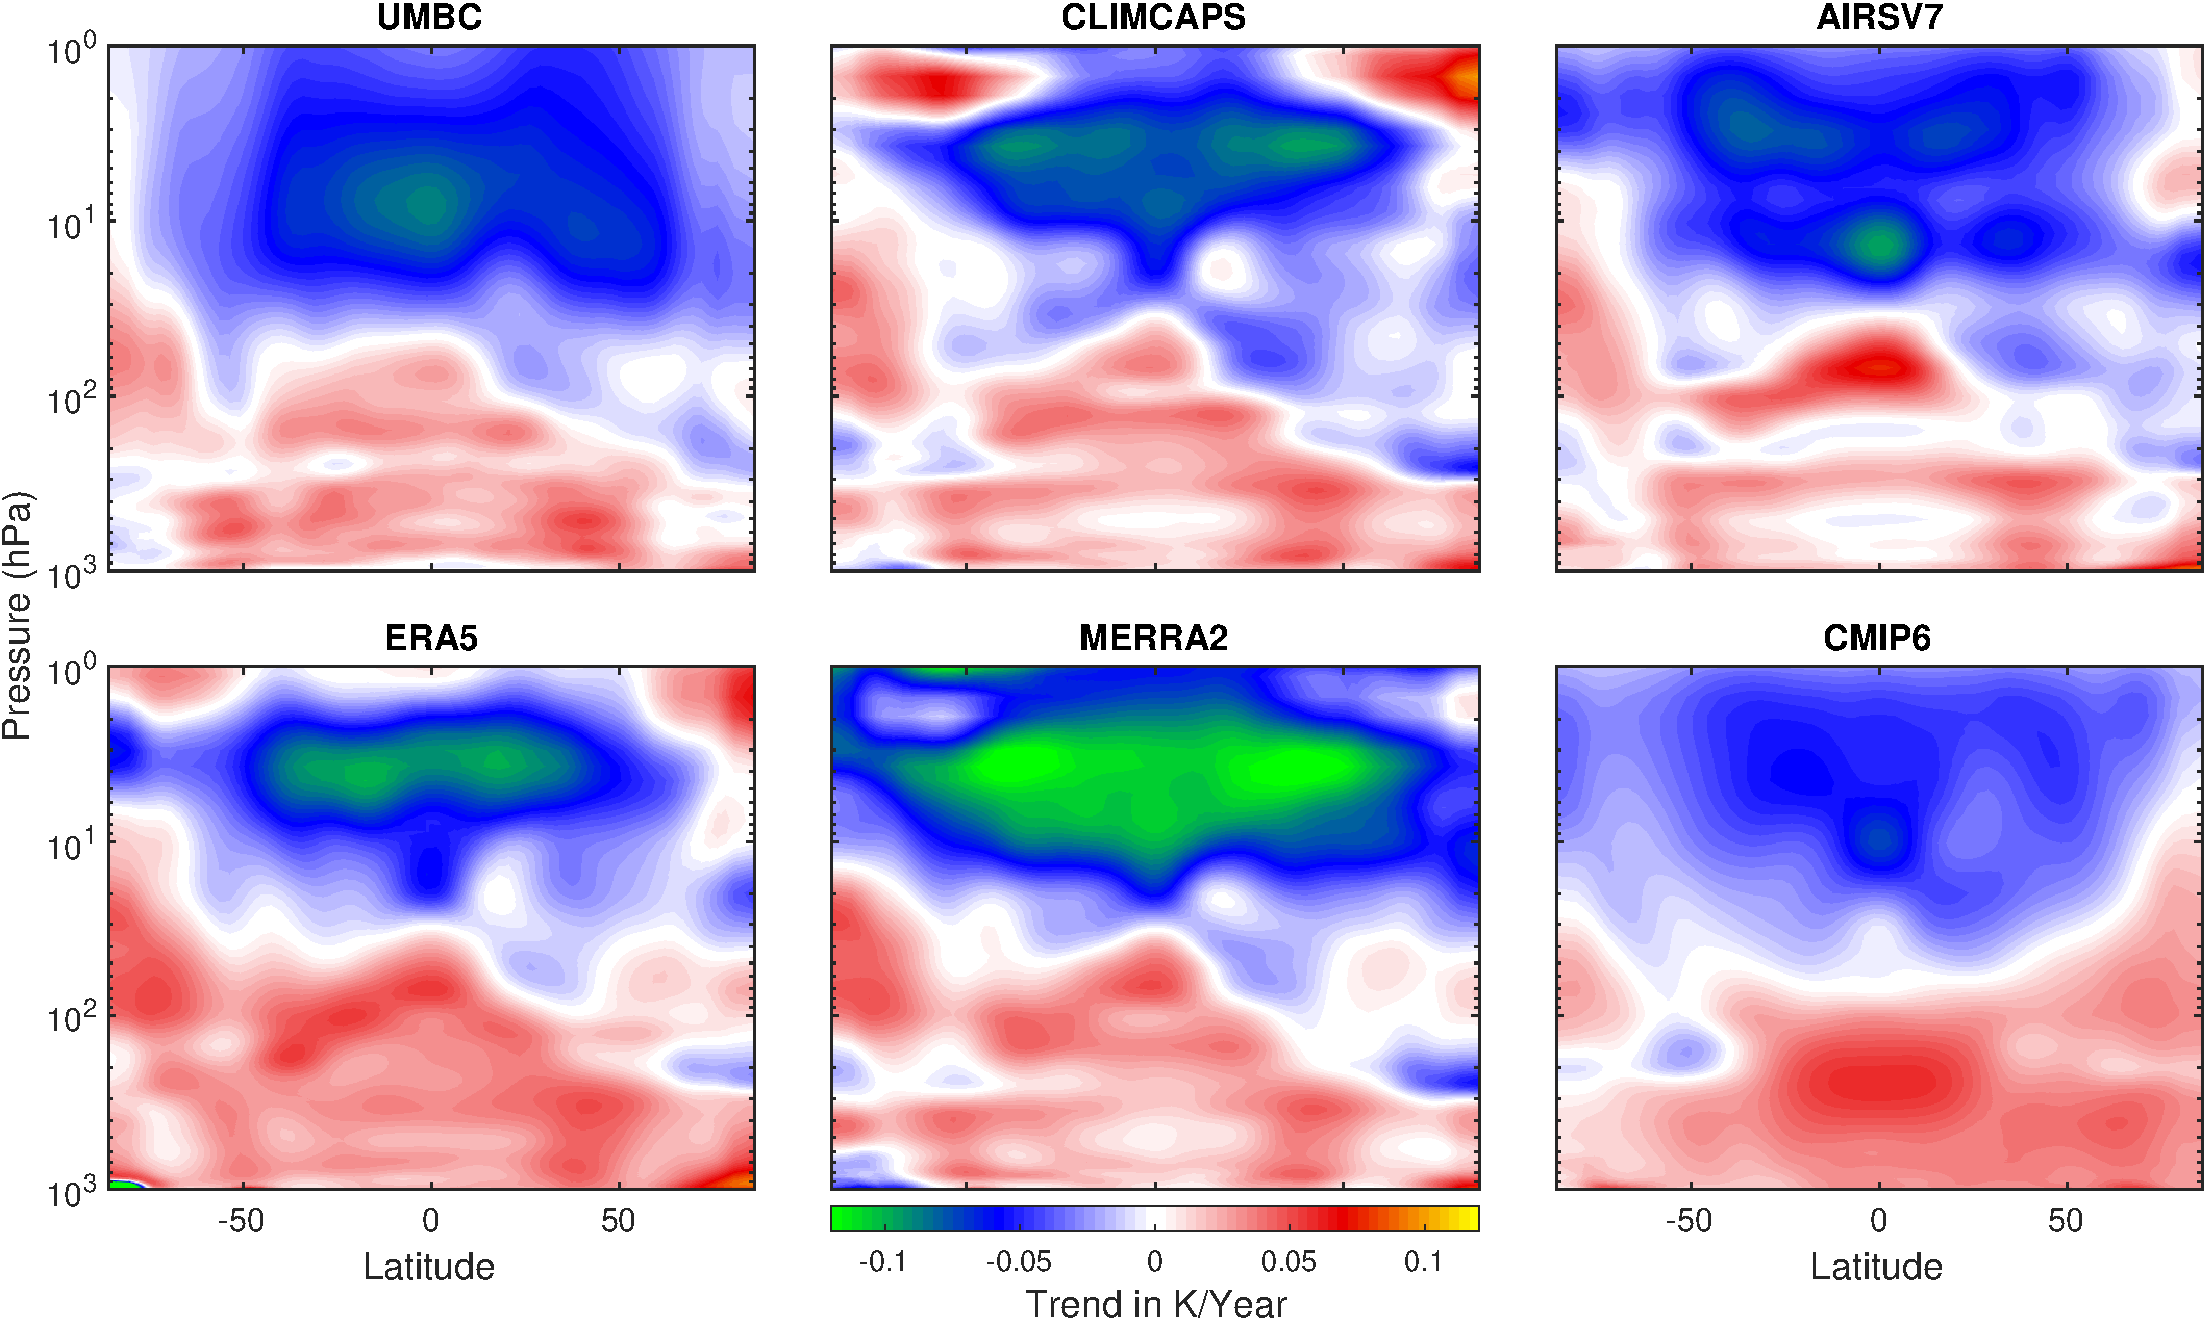
\includegraphics[width=\linewidth]{Strow_JPL_Apr2022/jpl_min//Figs/Pdf/zonal_trates_1to1000mbar_cmip6_newcaxis.pdf}
\end{center}

\footnotesize
IR does have null space near the tropopause.  But trends change sign there as well, as they should.\\
\vspace{0.1in}
UMBC uncertainties \textasciitilde{}0.01K/year (inter-annual variability)
\end{frame}

\begin{frame}[label={sec:org459ac58}]{Water Vapor Trends (with CMIP6 to 2014)}
\vspace{-0.15in}
\begin{center}
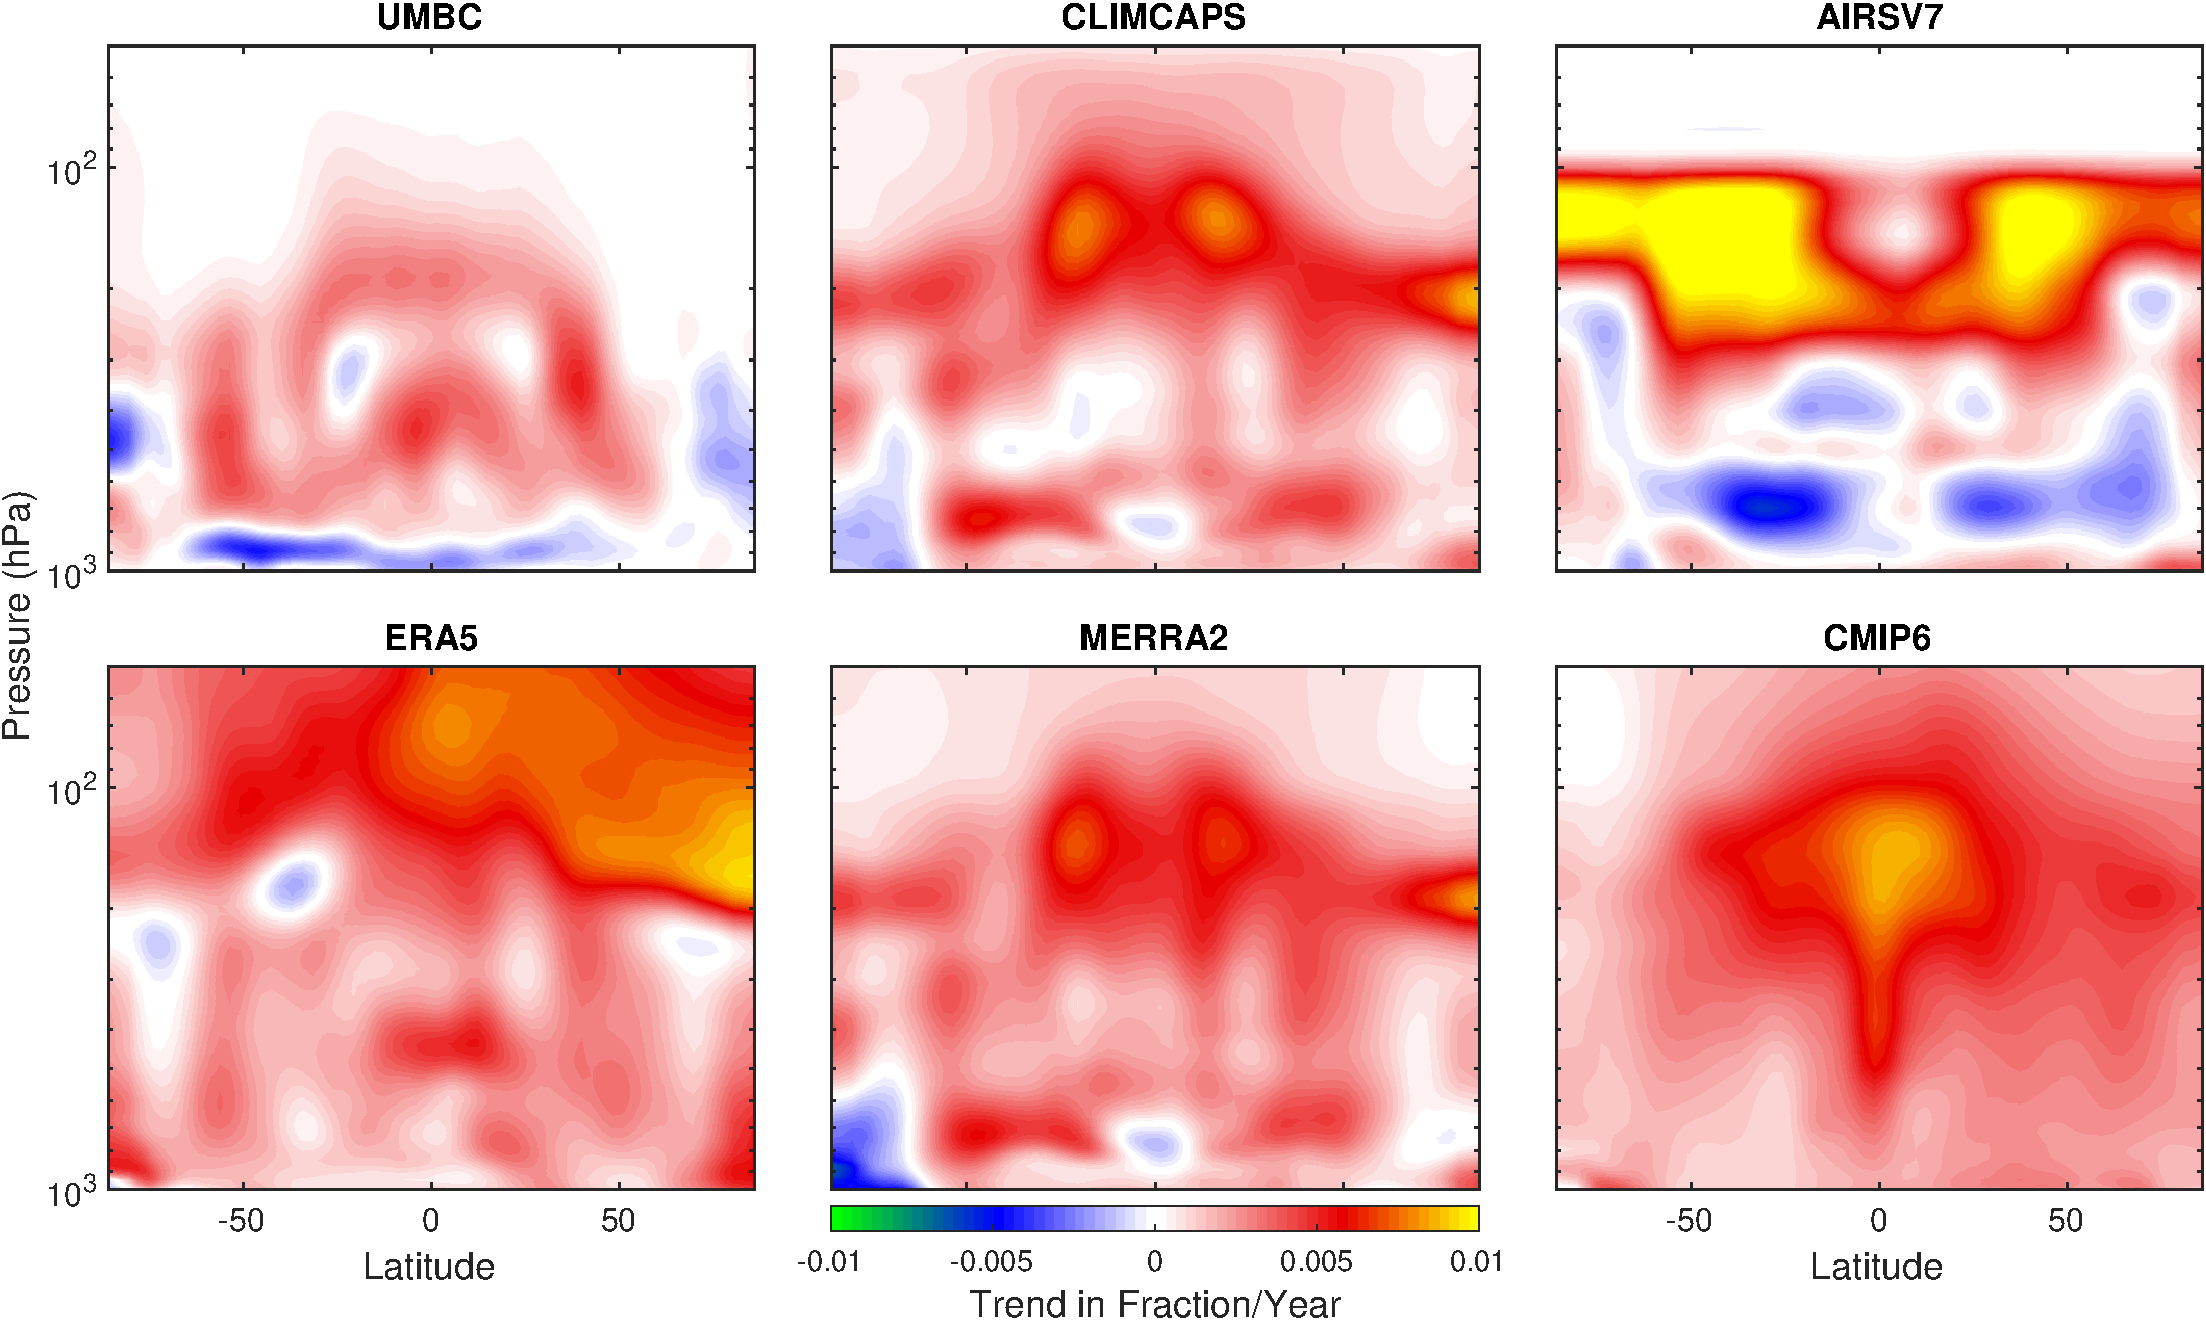
\includegraphics[width=\linewidth]{Strow_JPL_Apr2022/jpl_min//Figs/Pdf/zonal_wvrates_50to1000mbar_cmip6.pdf}
\end{center}

\small
\begin{itemize}
\item UMBC a-priori of zero influencing upper-trop WV
\item Quick test using MLS trends as a-priori for UMBC upper-trop
\end{itemize}
\end{frame}

%\begin{frame}[label={sec:org1e985f2}]{Water Vapor Trends (with AURA-MLS: from 2004+)}
%\vspace{-0.15in}
%\begin{center}
%\includegraphics[width=\linewidth]{Strow_JPL_Apr2022/jpl_min//Figs/Pdf/zonal_wvrates_50to1000mbar_mls_umbc_ap_mls.pdf}
%\end{center}
%\vspace{-0.1in}
%\small
%\begin{itemize}
%\item Quick test using MLS trends as a-priori for UMBC upper-trop
%\item MLS water vapor unimportant for OLR applications
%\item Mean global \(\Delta\) RH < 0.01\%/year
%\end{itemize}
%\end{frame}

\begin{frame}[label={sec:orgf7f9de9}]{Climate Feedback Estimation from Trend Retrievals}
\vspace{-0.15in}
\small
\begin{itemize}
\item CMIP period ends 2014 compared to our 2002-2021 time period
\item OLR differences directly from trends, no use of inter-annual variability for kernels
\item UMBC results similar to ERA-5 (not shown).
\item Cannot use MERRA2 surface T due to poor trends.
\end{itemize}

\vspace{-0.25in}
\begin{columns}
\begin{column}{0.5\columnwidth}
\begin{block}{\(\lambda\) WV}
\vspace{-0.1in}
\begin{center}
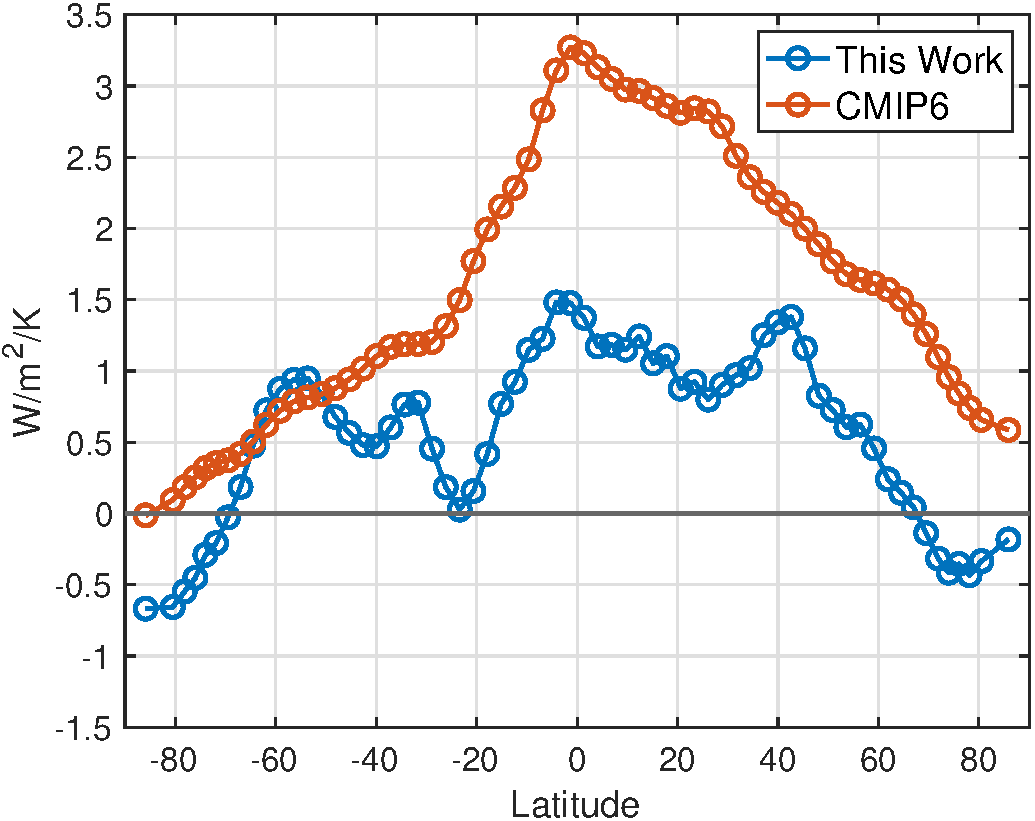
\includegraphics[width=\linewidth]{Strow_JPL_Apr2022/jpl_min//Figs/Pdf/wvlamda2.pdf}
\end{center}
\end{block}
\end{column}


\begin{column}{0.5\columnwidth}
\begin{block}{\(\lambda\) Lapse Rate}
\vspace{-0.1in}
\begin{center}
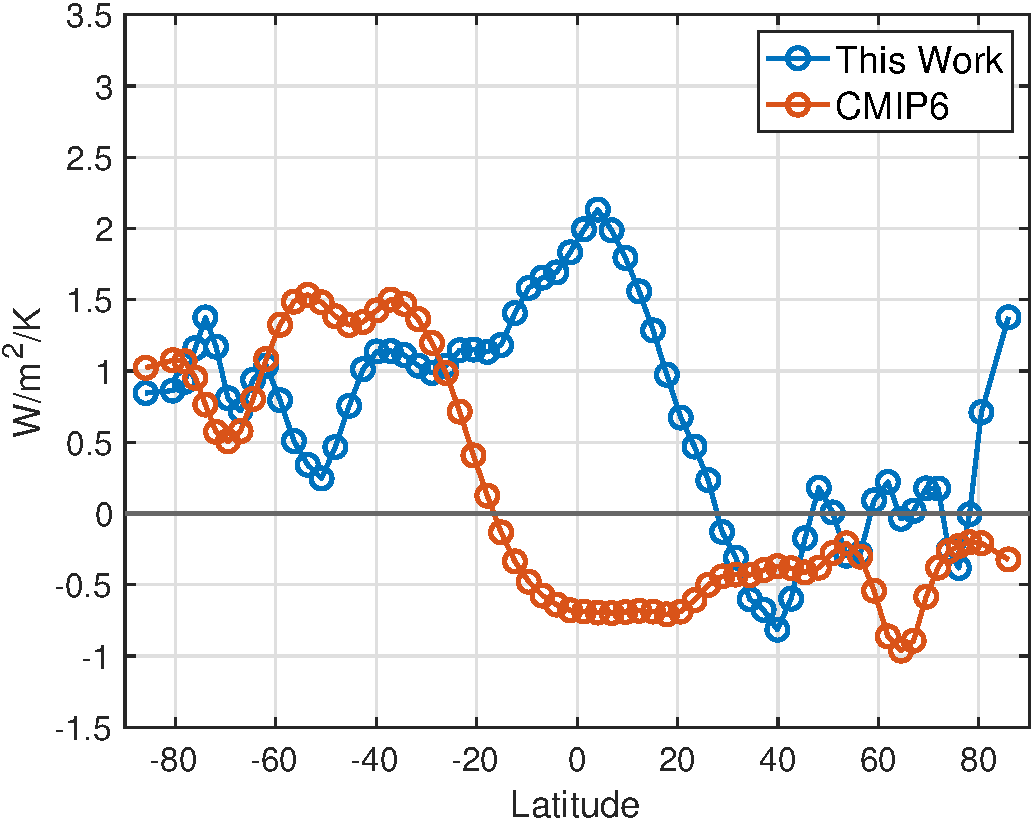
\includegraphics[width=\linewidth]{Strow_JPL_Apr2022/jpl_min//Figs/Pdf/lapselamda2.pdf}
\end{center}
\end{block}
\end{column}
\end{columns}

\vspace{-0.05in}
Note Positive lapse rate feedback in tropics for 2002-2022.
\end{frame}

\begin{frame}[label={sec:orgccfa059}]{OLR Clear Sky Trends from AIRS (UMBC version)}
\vspace{-0.1in}

\begin{columns}
\begin{column}{0.5\columnwidth}
\begin{block}{\small Total \(\Delta\) OLR (clear) over 19 Years}
\vspace{-0.1in}
\begin{center}
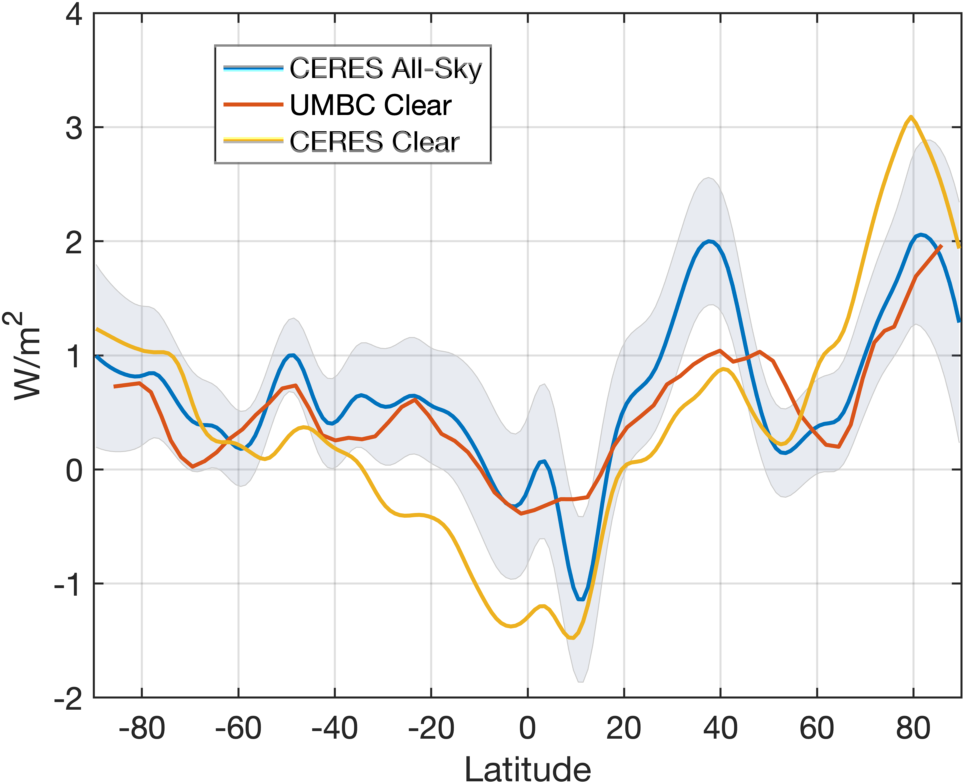
\includegraphics[width=\linewidth]{Strow_JPL_Apr2022/jpl_min//Figs/Png/ceres_clear_and_cld_19yrold_vs_umbc.png}
\end{center}
\end{block}
\end{column}

\begin{column}{0.5\columnwidth}
\begin{block}{\small Components from AIRS Trends}
\vspace{-0.1in}
\begin{center}
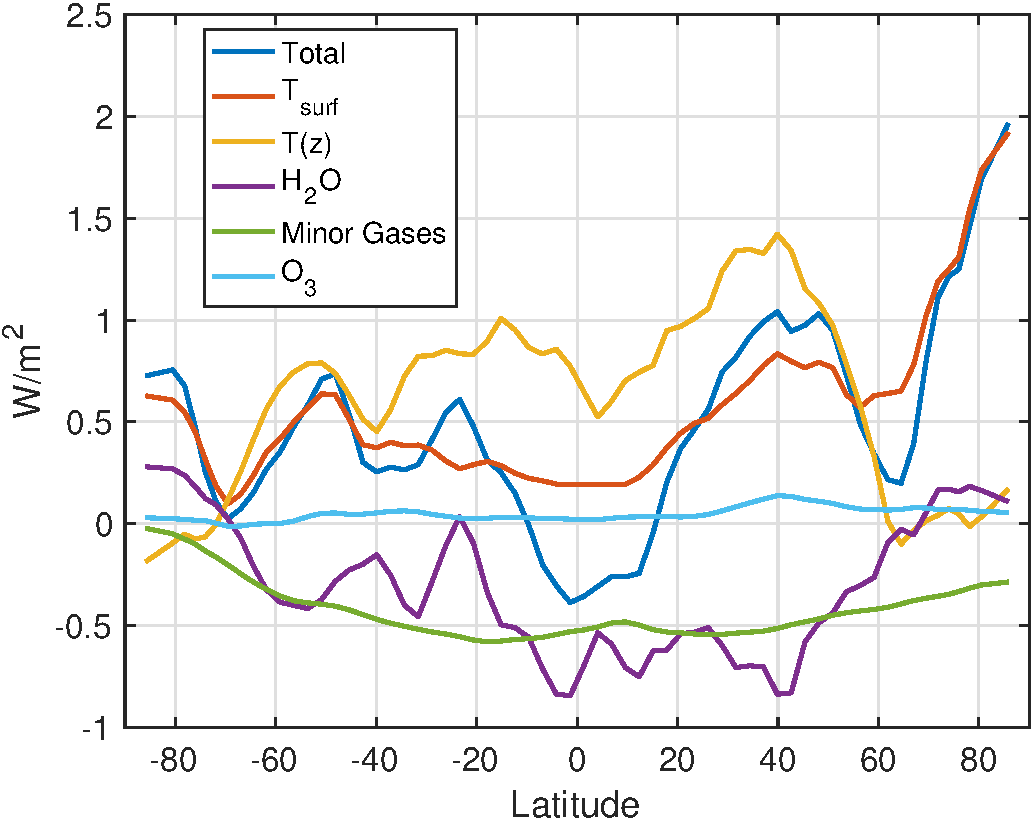
\includegraphics[width=\linewidth]{Strow_JPL_Apr2022/jpl_min//Figs/Pdf/umbc_olr_components.pdf}
\end{center}
\end{block}
\end{column}
\end{columns}

\vspace{-0.05in}

\begin{itemize}
\item UMBC clear closest to CERES All-Sky (but not perfect)
\item Hints for these differences seen in cloud forcing PDFs (in two slides)
\end{itemize}
\end{frame}

\begin{frame}[label={sec:org44223ad}]{Summary and Future}
\begin{itemize}
\item Hyperspectral IR observations are a unique dataset to monitor and understand climate change, for weather prediction and reanalysis, and to evaluate climate models

\item Hyperspectral IR radiances provide insights into the physics of the climate system that are not possible using broadband observations

\item We are starting to successfully merge hyperspectral IR radiances from different instruments which is critical for climate monitoring (GPSRO, MLS, MODIS/VIIRS)

\item We will continue to improve these merged products using more sophisticated approaches and including additional observations

\item But we need to keep these hyperspectral IR instruments alive and stable for as long as technically possible and continue to produce climate-level calibrated radiances
\end{itemize}
\end{frame}
\end{document}
